\documentclass{beamer}
\usepackage{tikz}
\usepackage{graphicx}
\usetikzlibrary{shapes.geometric, calc, positioning, arrows.meta}

\usetikzlibrary{positioning,shapes.geometric,backgrounds}
\usetikzlibrary{fit}
\usetikzlibrary {shapes.misc}

\usetikzlibrary {shadows,shapes.symbols}

\begin{document}

% Intro Slide
\begin{frame}
    \frametitle{What is a Protein Language Model?}
    
    % Explanation text
    \vspace{-1em}
    \begin{center}
        \textit{"A Protein Language Model uses patterns in protein sequences to predict structure, function, and behavior—like decoding the language of life."}
    \end{center}
    
    \vspace{2em}
    
    % Visual: Sequence -> Neural Network -> Prediction
    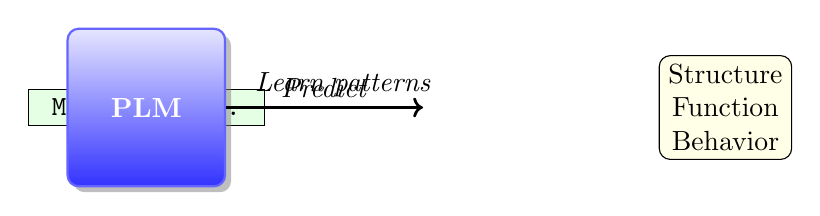
\begin{tikzpicture}[node distance=2.5cm, every node/.style={align=center}]
        % Protein sequence
        \node (seq) [rectangle, draw, minimum width=3cm, fill=green!10] 
        {\texttt{M E T A L ...}};
        
        % Arrow to Neural Network
        \draw[->, thick] (seq.east) -- ++(2,0) 
            node[midway, above] {\textit{Learn patterns}};
        
        % Neural network node
\node (nn) [rectangle,rounded corners, draw=blue!60, fill=blue!30, minimum size=2cm,
            shade, top color=blue!10, bottom color=blue!80, 
            text=white, thick, drop shadow={shadow xshift=0.5ex, shadow yshift=-0.5ex, opacity=0.5}] 
        {\textbf{PLM}};
        % Arrow to Prediction
        \draw[->, thick] (nn.east) -- ++(2.5,0) 
            node[midway, above] {\textit{Predict}};
        
        % Output predictions
        \node (pred) [rectangle, draw, rounded corners, fill=yellow!10, right=5cm of seq] 
        {Structure\\Function\\Behavior};
    \end{tikzpicture}
    
\end{frame}

\end{document}
